\documentclass{article}
\usepackage{tikz}
\usetikzlibrary{trees}

\begin{document}

\begin{tikzpicture}[
  level distance=15mm,
  every node/.style = {shape=circle, draw, minimum size=2mm},
  level 1/.style={sibling distance=60mm},
  level 2/.style={sibling distance=30mm},
  level 3/.style={sibling distance=15mm},
  edge from parent/.style={draw, thick},
  edge from parent fork down
]

\node (root) [fill=yellow] {1}
    child {node [fill=gray!50] {11}
        child {node [fill=black] {10}}
        child {node [fill=magenta] {14}}
        child {node [fill=pink] {3}}
        child {node [fill=red] {4}}
        child {node [fill=violet] {15}}
        child {node [fill=orange] {8}}
        child {node [fill=cyan] {5}}
        child {node [fill=green] {6}}
        child {node [fill=yellow] {9}}
        child {node [fill=blue] {2}}
        child {node [fill=orange] {13}}
        child {node [fill=green] {7}}
    }
    child {node [fill=yellow] {12}
        child {node [fill=red] {4}}
        child {node [fill=pink] {3}}
        child {node [fill=violet] {15}}
        child {node [fill=orange] {8}}
        child {node [fill=cyan] {5}}
        child {node [fill=green] {6}}
        child {node [fill=yellow] {9}}
        child {node [fill=blue] {2}}
        child {node [fill=orange] {13}}
        child {node [fill=green] {7}}
    }
    child {node [fill=yellow] {1}
        child {node [fill=black] {10}}
        child {node [fill=magenta] {14}}
        child {node [fill=pink] {3}}
        child {node [fill=red] {4}}
        child {node [fill=violet] {15}}
        child {node [fill=orange] {8}}
        child {node [fill=cyan] {5}}
        child {node [fill=green] {6}}
        child {node [fill=yellow] {9}}
        child {node [fill=blue] {2}}
        child {node [fill=orange] {13}}
        child {node [fill=green] {7}}
    };

\end{tikzpicture}

\end{document}